\definecolor{MATLABPurple}{RGB}{167, 9, 245}
\definecolor{MATLABBlue}{RGB}{14, 0, 255}

\section{Separable Filters}
\subsection{Creating a Convolution Mask}
\noindent In this section, we were given the following transfer function:

\begin{gather}
    \mathcal{H}_0(z_1, z_2) = \frac{1}{20.25}(z_1^{-1}z_2^{-1}+2.5z_1^{-1}+z_1^{-1}z_2+2.5z_2^{-1}+6.25+2.5z_2+z_1z_2^{-1}+2.5z_1+z_1z_2)
\end{gather}

Since this is a Linear Shift Invariant system, this transfer function can be implemented as a convolution between the input signal and a convolution mask. A mask can be generated simply by looking at the transfer function. First, we establish a few conventions. $z_1^0z_2^0$ will define the center of the convolution mask. Powers $z_1$ control the position of the coefficient in the first dimension relative to the center, with positive powers going down along the first dimension and negative powers going up along the first dimension. Similarly for $z_2$, but along the second dimension of the mask. Using these conventions we can generate the convolution mask that can be seen in eq \ref{eq:ConvMask} 

\begin{gather}
    ConvMask = \frac{1}{20.25}
    \begin{bmatrix}
            1.00 & 2.50 & 1.00 \\
            2.50 & 6.25 & 2.50 \\
            1.00 & 2.50 & 1.00 \\
    \end{bmatrix}
    \label{eq:ConvMask} 
\end{gather}

\subsection{Applying the Convolution Mask}
Applying the mask is simple. I called the MATLAB \textcolor{MATLABBlue}{\lstinline|conv2|} function passing in the image and the mask as inputs. It is important to note that the image should be normalized to be in the range [0-1] before passing it to \textcolor{MATLABBlue}{\lstinline|conv2|}. The output of the convolution can be seen in Figure \ref{fig:ConvdImageIO}

\begin{figure}[!h]
    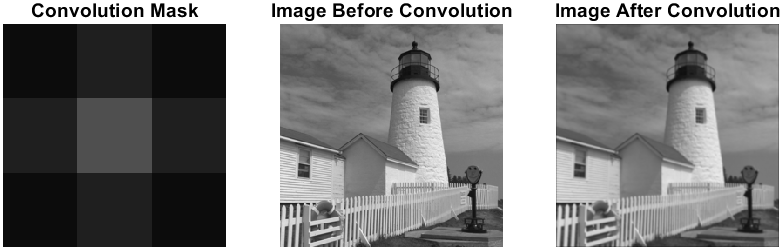
\includegraphics[width=1\textwidth]{ConvdImageIO.png}
    \centering
    \caption{Image before and after convolution. Mask is also shown.}
    \label{fig:ConvdImageIO}
\end{figure}

\subsection{Separating the Mask}
Applying the convolution mask was fairly easy. However, this operation is computationally expensive. Given an $M \times N$ image with an $R \times C$ convolution mask, we would need to perform $M \times N \times R \times C$ operations which can get expensive when considering large images and large masks. However, if we could apply a 1D mask to the rows and then another 1D mask to the columns and achieve the same output as the 2D mask, we could cut down the number of operations to $M \times N \times (R+C)$. Separable filters allow us to do this. A filter is considered to be separable if it can be written as the outer product of two vectors. That is to say, $mask \equiv u \otimes v \equiv uv^{\top}$ for a row vector $u$ and $v$. The mask in eq \ref{eq:ConvMask} can be decomposed into the following row and column vector.
\begin{equation}
    u = \frac{1}{4.5} 
    \begin{bmatrix}
        1.0 \\
        2.5 \\
        1.0 \\
    \end{bmatrix}
    \qquad
    v^{\top} = \frac{1}{4.5}
    \begin{bmatrix}
        1.0 & 2.5 & 1.0 \\
    \end{bmatrix}
\end{equation}
\pagebreak
We can perform the outer product of these two vectors to show that it gives the same result as the original mask

\begin{gather}
    \frac{1}{4.5}u \times \frac{1}{4.5}v = \frac{1}{4.5}\frac{1}{4.5}
    \begin{bmatrix}
        1.0 \\
        2.5 \\
        1.0 \\
    \end{bmatrix}
    \begin{bmatrix}
        1.0 & 2.5 & 1.0 \\
    \end{bmatrix}
\end{gather}

\begin{gather}
    \frac{1}{20.25}
    \begin{bmatrix}
        1.0 \times 1.0 & 1.0 \times 2.5 & 1.0 \times 1.0 \\
        2.5 \times 1.0 & 2.5 \times 2.5 & 2.5 \times 1.0 \\
        1.0 \times 1.0 & 1.0 \times 2.5 & 1.0 \times 1.0 \\
    \end{bmatrix}
\end{gather}

\begin{gather}
    \frac{1}{20.25}
    \begin{bmatrix}
        1.00 & 2.50 & 1.00 \\
        2.50 & 6.25 & 2.50 \\
        1.00 & 2.50 & 1.00 \\
    \end{bmatrix}
\end{gather}

\noindent Which we can clearly see is equal to eq \ref{eq:ConvMask} meaning that we can separate our 2D convolution mask into 2 smaller 1D convolution masks.

\subsection{Applying the Separated Masks}
To apply the separated masks we just need to call \textcolor{MATLABBlue}{\lstinline|conv2|} twice, with the output of the first convolution step being fed into the second convolution step and changing the mask from $u$ to $v$. Since we only care about the area where the image is defined, the padding option was set to \textcolor{MATLABPurple}{'same'}. This can be seen in Figure \ref{fig:SepConvIO}.

\begin{figure}[!h]
    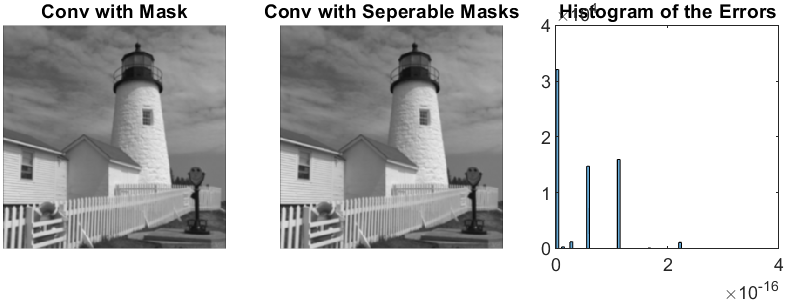
\includegraphics[width=1\textwidth]{SepConvdImageIO.png}
    \centering
    \caption{Image shown using 2D conv mask and separated masks. Histogram of errors is also shown}
    \label{fig:SepConvIO}
\end{figure}

\subsection{Calculating the Mean Absolute Error}
\noindent As we can see from the histogram, the absolute error is very low. The mean absolute error for the whole image was calculated to be $4.41691\mathrm{e}{-17}$.